%! Author = adnansiddiquei
%! Date = 13/12/2023

\subsection{Dataset A}\label{subsec:dataset-a}
\subsubsection{Question 1a}\label{subsubsec:q1a}
    \begin{figure}[htb]
    \centering
    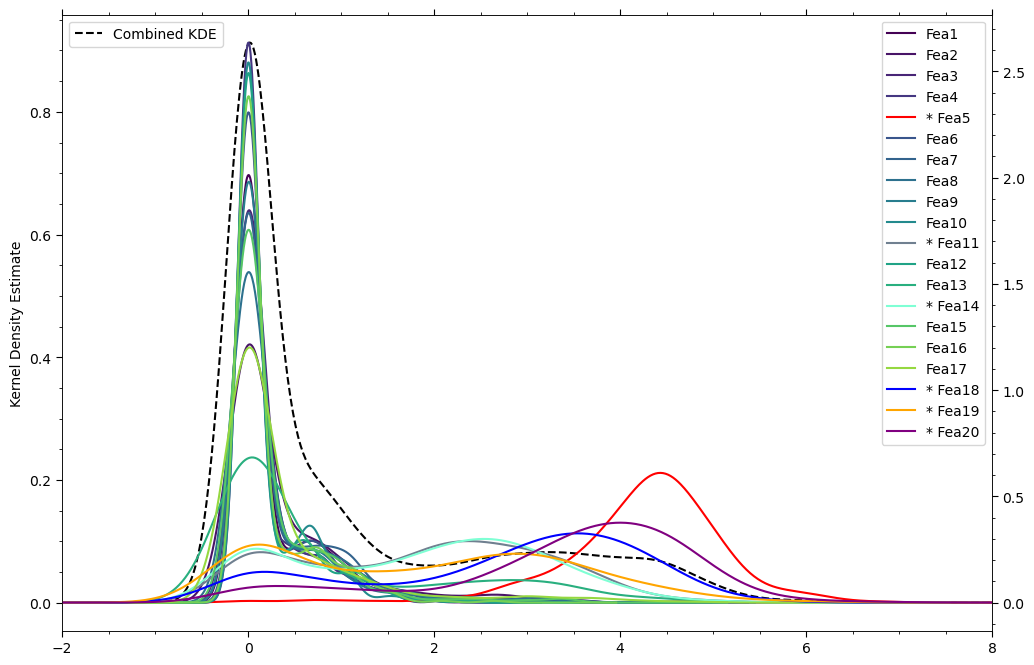
\includegraphics[width=0.9\textwidth]{./figures/q1a}
    \caption{A kernel density estimate of the first 20 features of the \inlinecode{A_NoiseAdded.csv} dataset, which has 20
    plots in total, with the legend and corresponding y-axis on the right. A combined KDE has also been plotted, with
    it's corresponding x-axis on the left. 7 of the 20 features have been highlighted in the legend with an asterisk,
    and have been coloured in slightly more contrasting colours and plotted with a dotted line. These features have a
    larger variance in their density, and are therefore more likely to be more discriminative.}
    \label{fig:q1a}
    \end{figure}

    Fig\eqref{fig:q1a} shows the combined and separated kernal density estimates of the first 20 features of the dataset.
    Several conclusions can be drawn from this plot.
    For most of the features, the KDE is concentrated around the zero value with very little variance, with the exception
    of 7 features: 5, 11, 13, 14, 18, 19 and 20.
    These features are likely to be more discriminative within classification algorithms, as they contain more variability.

\subsubsection{Question 1b}\label{subsubsec:q1b}

    \begin{figure}[htb]
    \centering
    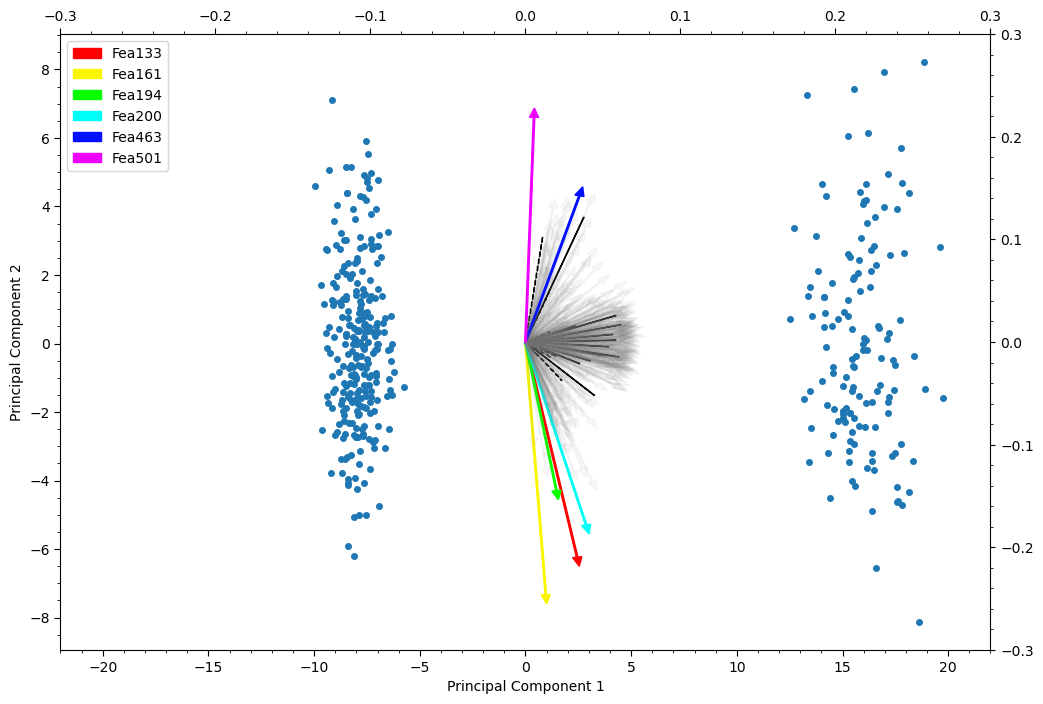
\includegraphics[width=0.9\textwidth]{./figures/q1b}
    \caption{A biplot of the first two principal components in the \inlinecode{A_NoiseAdded.csv} dataset.
        The coloured arrows indicate the first two principal component loading vectors for every feature which contributes to
        either principal component more than 2\%, these are the most discriminative features.
        Every other loading vector has been plotted in very light grey so their general directions and magnitudes are
        visible.
        The loading vectors for the first 20 features have also been plotted in darker black lines, with the dotted
        black lines corresponding to the dotted KDEs in Fig\eqref{fig:q1a}.
        The loading vectors use the right and top axis of the plot.
        The blue dots indicate the scores for each observation in the dataset for the first two principal components.
        The scores use the left and bottom axis of the plot.
        All four axis are symmetric about the origin for ease of comparison.}
    \label{fig:q1b}
    \end{figure}

    The biplot in Fig\eqref{fig:q1b} shows a PCA of the entire dataset, after standardisation has been applied to each
    feature.
    The coloured arrows indicate the loadings of the features which contribute more than 2\% to either principal
    component, which implies that none of the first 20 features are particularly discriminative.
    An interesting observation is that the most discriminative features are very disciminative with respect to the
    second principal component, whereas the less discriminative features (of which there are many, many more of) are
    more discriminative with respect to the first principal component.
    As a result, the scores on the biplot for the observations w.r.t. the first two principal components separate the
    observations more along the first principal component, rather than the second.

\subsubsection{Questions 1c and 1d}\label{subsubsec:q1cd}
    \begin{figure}[htb]
    \centering
    \begin{subfigure}[b]{0.9\linewidth}
        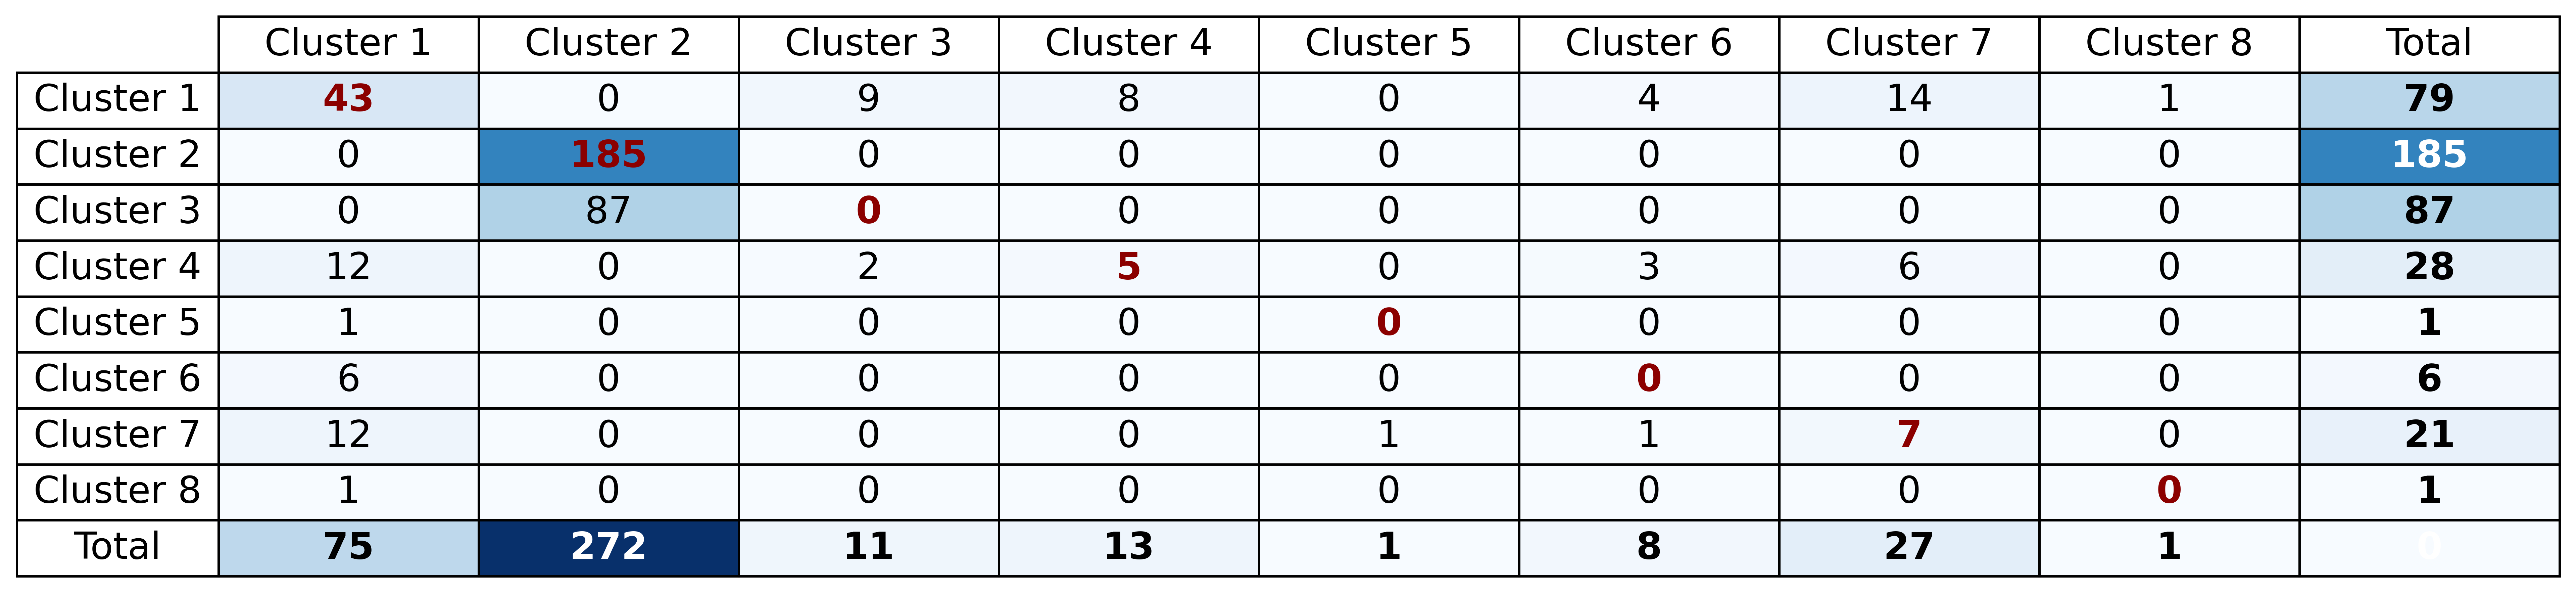
\includegraphics[width=1\textwidth]{./figures/q1c}
        \caption{A contingency table for two k-means clusterings of the \inlinecode{A_NoiseAdded.csv} dataset, with $k=8$,
            the default \inlinecode{scikit-learn} value. 240 of the 408 observations lie on the leading diagonal.}
        \label{fig:q1c}
    \end{subfigure}
    \hfill
    \begin{subfigure}[b]{0.9\linewidth}
        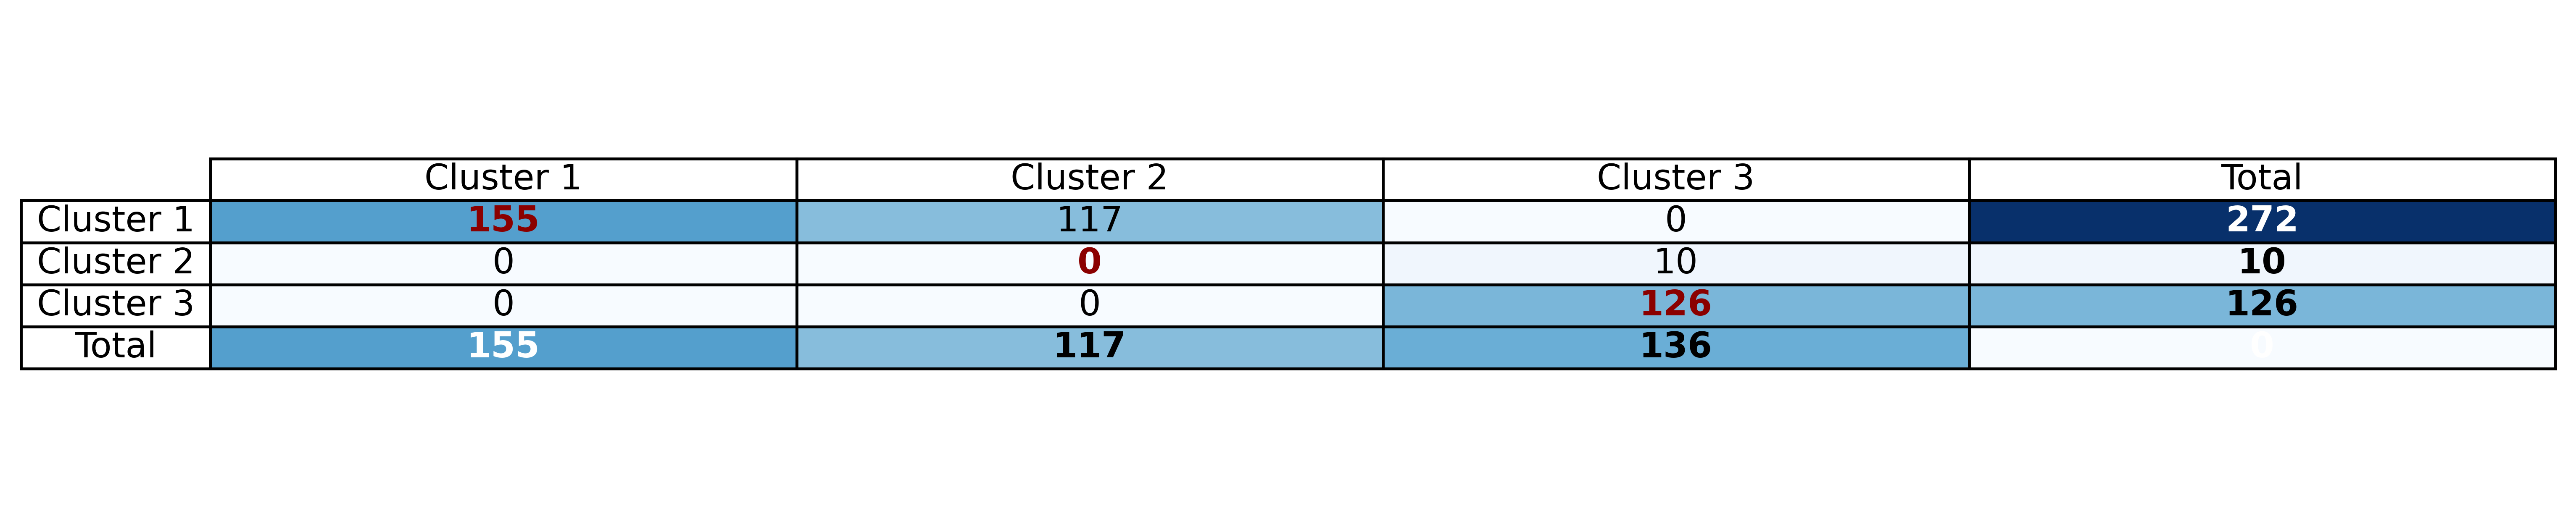
\includegraphics[width=1\textwidth]{./figures/q1d}
        \caption{A contingency table for two k-means clusterings of the \inlinecode{A_NoiseAdded.csv} dataset, with $k=3$.
            281 of the 408 observations lie on the leading diagonal.}
        \label{fig:q1d}
    \end{subfigure}
    \caption{Contingency tables for two k-means clusterings of the \inlinecode{A_NoiseAdded.csv} dataset with number of
        clusters $k=3$ and $k=8$.
        Each feature in the dataset was standardised before clustering.
        \inlinecode{kmeans_1} totals are on the right and \inlinecode{kmeans_2} totals are on the bottom.}
    \label{fig:q1cd}
    \end{figure}

    Fig\eqref{fig:q1c} shows the contingency table for two k-means clusterings of the dataset with $k=8$ and $k=3$.
    The two clusterings (\inlinecode{kmeans_1} and \inlinecode{kmeans_2}) were formed by training two k-means models on
    half of the dataset, and then the other half were mapped onto the learned clusters.
    Standardisation was applied to each feature before clustering as k-means is sensitive to feature scaling, this is because
    k-means works by computing a centroid for each cluster such that the sum of the squared Euclidean distances between
    each centroid and the observations in the cluster is minimised.
    Therefore, without standardisation, features with larger variances and scale will dominate the clustering.
    Predictions are then made by assigning new observations to the cluster whose centroid is closest to the
    observation \cite{sklearn-k-means}.
    Crucially, the labels assigned to each cluster from each k-means computation are arbitrary, therefore, the labels
    in \inlinecode{kmeans_2} were mapped back to the labels in \inlinecode{kmeans_1} by finding which centroids in each
    clustering were closest to each other.
    This step was crucial, otherwise the contingency table would be meaningless.

    For $k=8$, 59\% of the observations lie on the leading diagonal, which indicates that the two clusterings were not very
    similar or stable, as a large proportion of the observations were assigned to different clusters in each clustering.
    \inlinecode{kmeans_1} clustered 85\% of the observations into clusters 1, 2 and 3.
    \inlinecode{kmeans_2} clustered 86\% of the observations into clusters 1 and 2.
    This indicates that both clusterings identified most of the data lives within a small set of clusters, which was
    expected as the dataset is labelled and so it is known that there are only 3 clusters - both clusterings identified
    at least 2 similar clusters (1 and 2).
    However, the presence of very small clusters indicates that there may be outliers present in the dataset or smaller
    clusters that the large $k=8$ is overfitting to.

    Fig\eqref{fig:q1d} shows the contingency table for two k-means clusterings of the dataset with $k=3$.
    A larger proportion of the observations lie on the leading diagonal compared to $k=8$, which is expected because
    the number of clusters is both smaller and equal to the actual number of clusters in the dataset.
    \inlinecode{kmeans_2} identified 3 distinct clusters whereas \inlinecode{kmeans_1} only identified 2 distinct
    clusters with a few remnant observations in assigned to cluster 2.

\subsubsection{Questions 1e}\label{subsubsec:q1e}
    \begin{figure}[htb]
    \centering
    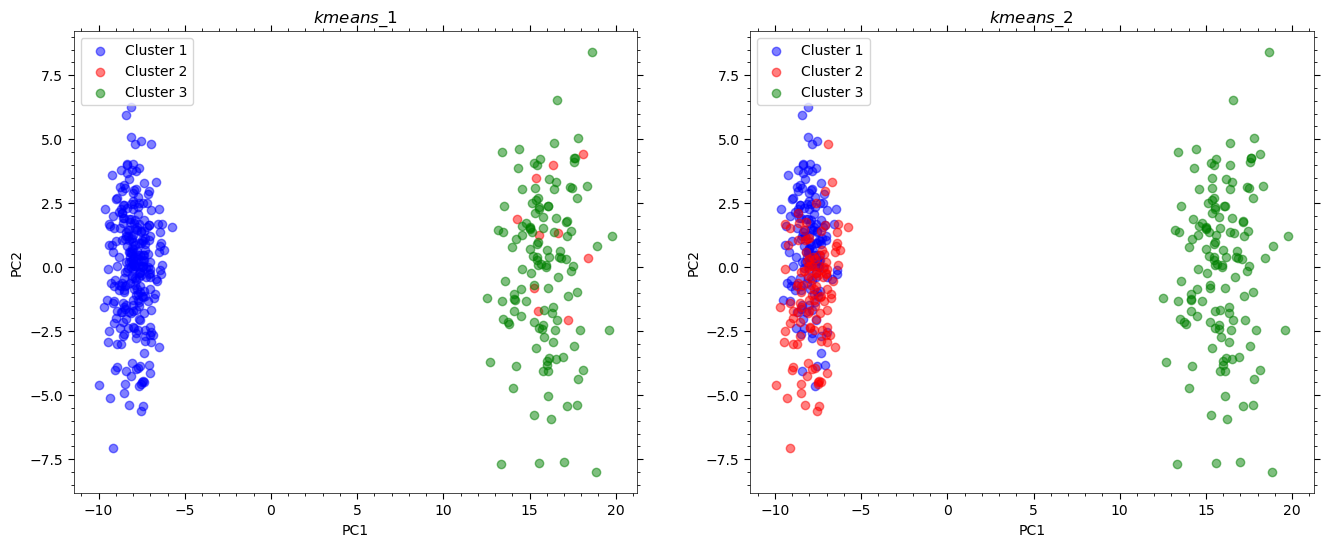
\includegraphics[width=1\textwidth]{./figures/q1e}
    \caption{The k-means clusterings performed with $k=3$, shown on the contingency table in Fig\eqref{fig:q1d}, plotted
        on the first two principal components of the dataset shown in Fig\eqref{fig:q1b}. The left plot is
        \inlinecode{kmeans_1} and the right plot is \inlinecode{kmeans_2}.}
    \label{fig:q1e}
    \end{figure}

    Fig\eqref{fig:q1e} shows the k-means clusterings on the PCA plot shown in Fig\eqref{fig:q1b}.
    The PCA indicates that there are two clusters in the dataset when it is reduced to the first two principal components
    (which generally explain a large amount of the variance in a dataset).
    Fig\eqref{fig:q1e} provides subtle evidence in favour of this as well, note that clusters 1 and 3 are stable, but cluster
    2 jumps between the two groups in the PCA plots, whilst only capturing observations from either one of the groups
    but never both.
    The fact that cluster 2 never captures data from both groups in the PCA plot indicates that it is likely capturing
    a subset of the data from one of the PCA groups, based on random initialisation of the k-means algorithm.
    Its inability to capture data from both PCA groups at once, and the clear separation of clusters 1 and 3 indicate
    that there may only be two clusters in the dataset, as opposed to the three clusters that the labels indicate.

    Performing k-means before PCA has the advantage of being able to visualise the clusters separation in the original
    feature space, whilst performing PCA before k-means has the advantage of being able to reduce computational load
    and identify clusters along the first two principal components (which often explain the most variance in the dataset).
    Performing PCA first also provides a visual way to determine the number of clusters in the dataset if is is unknown as
    PCA will separate data along the two most discriminative axis.
    If the number of clusters is unknown, performing PCA first would be a good idea.
    As to which is better, it can depend on the dataset and the number of features.
    It can often turn out that the first two principal components do not actually explain much of the variance, and as
    such, in these cases it can be better to perform k-means first.
